\documentclass[a4paper,14pt]{extarticle}
\usepackage[utf8]{inputenc}
\usepackage[russian]{babel}
\usepackage{graphicx}
\usepackage[top=0.8in, bottom=0.8in, left=0.8in, right=0.8in]{geometry}
\usepackage{pgfplots}
\usepackage{amsmath}
\usepackage{setspace}
\usepackage{titlesec}
\usepackage{float}
\usepackage{chngcntr}
\usepackage{pgfplots}
\usepackage{amsfonts}
\usepackage{pgfplotstable}
\usepackage{multirow}
\usepackage{karnaugh-map}
\usepackage{tikz,xcolor}
\usepackage{listings}

\titleformat{\section}[hang]
  {\bfseries}
  {}
  {0em}
  {\hspace{-0.4pt}\large \thesection\hspace{0.6em}}
  
  
\titleformat{\subsection}[hang]
  {\bfseries}
  {}
  {0em}
  {\hspace{-0.4pt}\large \thesubsection\hspace{0.6em}}

\newcommand{\nx}{\overline{x}}
\newcommand{\p}{0.31}
\newcommand{\scale}{1.4}

\counterwithin{figure}{section}
\counterwithin{equation}{section}
\counterwithin{table}{section}

\lstdefinestyle{CStyle}{
    basicstyle=\footnotesize,
    breakatwhitespace=false,         
    breaklines=true,                 
    captionpos=b,                    
    keepspaces=true,                 
    numbers=left,                    
    numbersep=5pt,                  
    showspaces=false,                
    showstringspaces=false,
    showtabs=false,                  
    tabsize=2,
    language=C
}

\begin{document}
\begin{titlepage}
\centering
\small Балтийский государственный технический университет «Военмех» им. Д.Ф.Устинова \\
\vspace{3cm}
\normalsize Кафедра И5\\
«Информационные системы и программная инженерия»\\
\vspace{3cm}
\textbf{Практическое задание №5}\\
по дисциплине Основы программирования на тему\\ 
\textbf{«Функции»}\\
\vfill

\begin{flushleft}
\textbf{Выполнил:}
\hfill {Мальцев А.С.} \\
\hfill {Группа И595} \\
\vspace{1cm}
\textbf{Преподаватель:}
\hfill {Лазарева Т.И.} \\
\end{flushleft}
\vspace{3cm}

{\centering Санкт-Петербург \\ 
\vspace{0.15cm}
2019}
\end{titlepage}

\setcounter{page}{2}
\section{Цель работы}
Научиться использовать функции для выполнения однотипных действий над различными данными, правильно задавать параметры функций, передавать указатели на функции в качестве параметров.

\section{Ход работы}
\subsection{Файл io.c, в котором содержатся функции ввода и вывода массива}
\begin{center}
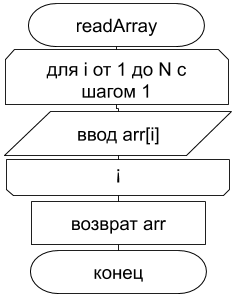
\includegraphics[scale=0.6]{lab5-io-1.png}
\hspace{2cm}
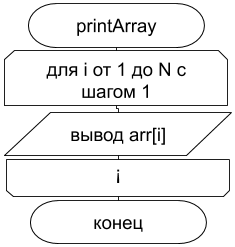
\includegraphics[scale=0.6]{lab5-io-2.png}\\
Схема программы
\end{center}
\lstinputlisting[language=c, frame=single, style=CStyle]{../io.c}
\begin{center}
Текст программы\\
\end{center}

\subsection{Задание 1}
Поменять местами первый максимальный элемент массива А (5) и последний максимальный элемент массива В (7).\\
\textit{Исходные данные:} входные значения могут быть любыми, поэтому массивы A и B типа double.\\
\textit{Дополнительные переменные:} указатели m1 и m2 для хранение ссылок на максимальные элементы массивов.\\
\textit{Результирующие данные:} дополнительных переменных для вывода не требуется.\\
\begin{center}
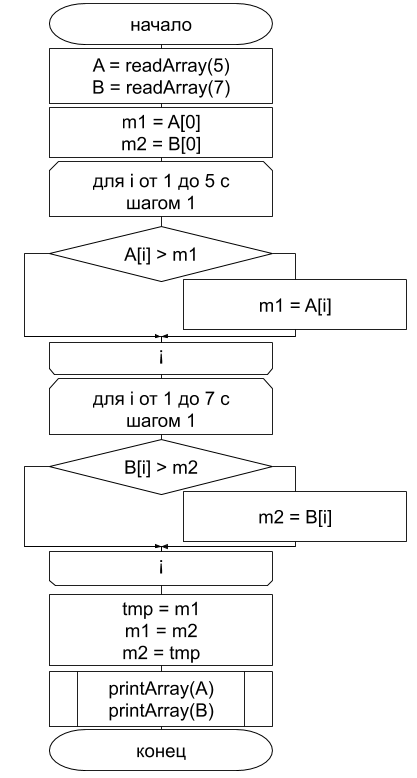
\includegraphics[scale=0.6]{lab5-1.png}\\
Схема программы
\end{center}
\lstinputlisting[language=c, frame=single, style=CStyle]{../1.c}
\begin{center}
Текст программы\\
\vspace{0.6cm}
\begin{tabular}{|l|l|}
\hline
\multicolumn{1}{|c|}{Исходные данные}& \multicolumn{1}{|c|}{Вывод программы}\\
\hline
A = 1 2 3 4 5 & A = 1 2 3 4 7 \\
B = 1 2 3 4 5 6 7 & B =1 2 3 4 5 6 5 \\
\hline
A = 4 23 99 4 72 & A = 4 23 44 4 72 \\
B = -55 32 7 9 0 2 44 & B = -55 32 7 9 0 2 99 \\
\hline
\end{tabular}\\
\vspace{0.3cm}
Результаты тестирования
\end{center}

\subsection{Задание 2}
Даны два вектора: Y (30) и X (30). Вычислить значение функции\\ $ \displaystyle\frac{n\sum x_{i}y_{i} - \sum x_{i} \sum y_{i}}{\sqrt{(n \sum x_{i}^{2} - (\sum x_{i})^{2})(n \sum y_{i}^{2} - (\sum y_{i})^{2})}} $. Сумму элементов одного массива и сумму квадратов элементов одного массива оформить отдельными функциями.\\
\textit{Исходные данные:} входные значения могут быть любыми, поэтому массивы X, Y и n типа double.\\
\textit{Результирующие данные:} f типа double для вывода значения функции.\\
\begin{center}
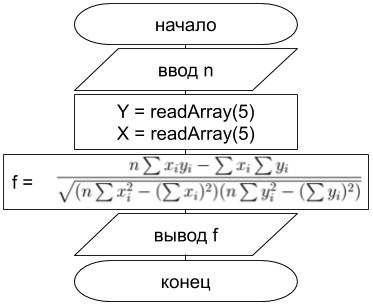
\includegraphics[scale=0.6]{lab5-2.png}\\
\vspace{0.3cm}
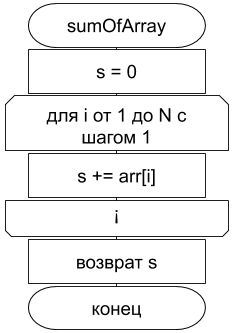
\includegraphics[scale=0.6]{lab5-2-1.png}
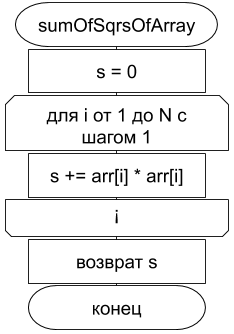
\includegraphics[scale=0.6]{lab5-2-2.png}
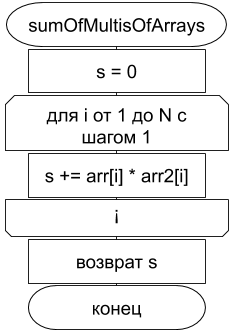
\includegraphics[scale=0.6]{lab5-2-3.png}\\
Схема программы
\end{center}
\lstinputlisting[language=c, frame=single, style=CStyle]{../2.c}
\begin{center}
Текст программы\\
\vspace{0.6cm}
\begin{tabular}{|l|l|}
\hline
\multicolumn{1}{|c|}{Исходные данные}& \multicolumn{1}{|c|}{Вывод программы}\\
\hline
n = 4 & f = -17.000000 \\
Y = 1 2 3 4 5 & \\
X = 5 4 3 2 1 & \\
\hline
n = 20 & f = 0.133900 \\
Y = -1 5 98 3 7 & \\
X = 4 7 8 22 56 & \\
\hline
\end{tabular}\\
\vspace{0.3cm}
Результаты тестирования
\end{center}

\subsection{Задание 3}
$ \displaystyle\int_{-1}^4 2x(x^2+1) dx , \displaystyle\int_{0,5}^{3,5} \frac{e^{2x}}{2x} dx, N = 30 $, метод Ньютона.\\
\textit{Исходные данные:} входных данных нет.\\
\textit{Результирующие данные:} дополнительной переменной не требуется.\\
\begin{center}
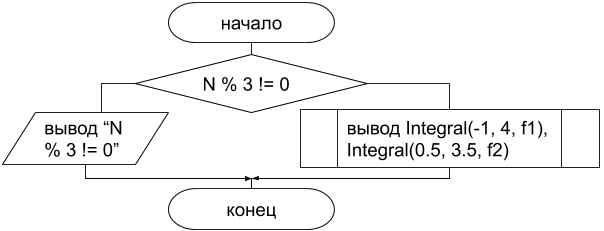
\includegraphics[scale=0.6]{lab5-3.png}\\
\vspace{0.3cm}
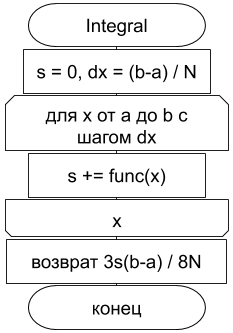
\includegraphics[scale=0.6]{lab5-3-1.png}
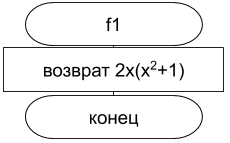
\includegraphics[scale=0.6]{lab5-3-2.png}
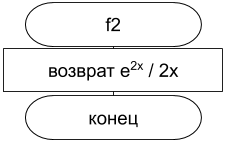
\includegraphics[scale=0.6]{lab5-3-3.png}\\
Схема программы
\end{center}
\lstinputlisting[language=c, frame=single, style=CStyle]{../3.c}
\begin{center}
Текст программы\\
\vspace{0.6cm}
\begin{tabular}{|l|}
\hline
\multicolumn{1}{|c|}{Вывод программы}\\
\hline
142.250000 89.033025 \\
\hline
\end{tabular}\\
\vspace{0.3cm}
Результаты тестирования
\end{center}


\end{document}
